\documentclass[12pt]{scrartcl}

% Font and input encoding
\usepackage{fontspec}
\defaultfontfeatures{Ligatures=TeX,Renderer=Basic}
\usepackage{polyglossia}
\setmainlanguage{russian}
\setotherlanguage{english}

% Explicitly setting fonts that support Cyrillic
\setmainfont{CMU Serif}
\setsansfont{CMU Sans Serif}
\setmonofont{CMU Typewriter Text}

% For math symbols
% Include AMS packages for mathematical symbols and fonts
\usepackage{amsmath}
\usepackage{amssymb}

% For code listings
\usepackage{listings}

% For tables
\usepackage{tabularx}
\usepackage{placeins}

% For images
\usepackage{graphicx}
\usepackage{float}

% For drawing
\usepackage{tikz}
\usepackage{pgfplots}
\pgfplotsset{compat=1.18}
\usepackage{pgfplotstable}
\usetikzlibrary{pgfplots.statistics}
\usetikzlibrary{pgfplots.groupplots} % Load the groupplots library

% For files reading
\usepackage{filecontents}


% Bibliography management (optional in presentation, often omitted)
\usepackage[backend=biber]{biblatex}
\addbibresource{references.bib} % Specify your bibliography file here

% For clickable links (often less necessary in presentations)
\usepackage{hyperref}

% Settings for links (optional in presentations)
\hypersetup{
	colorlinks=true,
	linkcolor=red,
	filecolor=magenta,
	urlcolor=cyan,
}

% Document metadata
\title{Автоматизированное практическое применение метода балансировки матриц Брэгмана в варианте алгоритма Синкхорна\,--\,Кноппа для риск-ориентированной оценки страховой стоимости объектов недвижимости}
\subtitle{\foreignlanguage{english}{Practical application of the Bregman matrix balancing method in a variant of the Sinkhorn-Knopp algorithm for risk-oriented estimation of insurance value of real estate objects}}

% Define authors
\author{К.\,А.~Мурашев\thanks{email: kirill.murashev@gmail.com, \href{https://t.me/AIinValuation}{Telegram}, директор ООО ``Совконсалт'', член Комитета по Научным и Методическим Вопросам Оценочной Деятельности Национального Объединения СРО Оценщиков ``Союз СОО''}}

\date{\today}

\begin{document}

\maketitle

\begin{abstract}
Точная оценка стоимости здания имеет решающее значение для страховых сделок, позволяя сбалансировать сбор премии и риск для страховщиков, а также обеспечить соблюдение нормативных требований. Использование затратного подхода для определения страховой стоимости на основе восстановительной самом по себе не представляет какую-либо сложность. Однако оно может приводить к завышению стоимости, что может дать возможность для совершения страхового мошенничества или непреднамеренного завышения стоимости. Это несоответствие возникает из-за неразрывной связи земли и здания в сделках с недвижимостью, что затрудняет определение истинной справедливой стоимости одного здания. Точный учёт функционального устаревания и внешнего обесценения в рамках затратного подхода весьма затруднён без внешних рыночных данных, получение которых чаще всего крайне затруднено. Существующие решения, такие как типовые предельные значения, лишены гибкости и могут привести к недоплате страховых взносов или чрезмерному принятию риска. Для решения этих проблем в данной работе предлагается новый способ, сочетающий сравнительный подход для оценки единого объекта недвижимости, а также затратный подход для определения восстановительной стоимости с методом балансировки матриц Брэгмана в реализации посредством алгоритма Синкхорна-Кноппа. Используя рыночные данные о совокупной стоимости земли и здания, а также оценку стоимости здания на основе затрат, возможно получить справедливый верхний предел страховой стоимости. Приведённый практический пример демонстрирует вычислительную эффективность и простоту этого способа, показывая его потенциал для повышения точности, предотвращения мошенничества и обеспечения справедливости в процессе оценки страховой стоимости.


\bigskip
\textenglish{Accurate assessment of building value is crucial for insurance transactions, balancing premium collection and risk for insurers, while ensuring regulatory compliance. While the cost approach is commonly used for valuation, it may underestimate market value, leading to potential fraud or unintentional overvaluation. This discrepancy arises from the inherent inseparability of land and building in real estate transactions, making it challenging to isolate the building's true market value. Furthermore, accurately accounting for functional obsolescence and external impairment within the cost approach can be difficult without external market insights, potentially exploited for fraudulent overvaluation. Current solutions, like typical limit values, lack flexibility and can result in underpayment of premiums or excessive risk acceptance. To address these issues, this paper proposes a novel method combining the market approach for valuing a single real estate object and the cost approach for determining the replacement value with the Bragman matrix balancing method as implemented through the Synhorn-Knopp algorithm. By leveraging market data on combined land and building values, along with cost-based building value estimates, we derive a fair insurance value ceiling, mitigating both undervaluation and overvaluation risks. A practical case study demonstrates the implementation and effectiveness of this method, showcasing its potential to enhance accuracy, deter fraud, and promote fairness in the insurance valuation process.}

\end{abstract}

\section{Введение}\label{sec:Introduction}
В соответствии с п.~2 ст.~947 Гражданского Кодекса России~\cite{GKRFP2},\emph{ при страховании имущества или предпринимательского риска, если договором страхования не предусмотрено иное, страховая сумма не должна превышать их действительную стоимость (страховой стоимости). Такой стоимостью считается: для имущества его действительная стоимость в месте его нахождения в день заключения договора страхования}$\ldots$. В соответствии с п.~1 ст.~951 того же Кодекса, \emph{если страховая сумма, указанная в договоре страхования имущества или предпринимательского риска, превышает страховую стоимость, договор является ничтожным в той части страховой суммы, которая превышает страховую стоимость}. В соответствии с п.~1 ст.~945 того же Кодекса, \emph{при заключении договора страхования имущества страховщик вправе произвести осмотр страхуемого имущества, а при необходимости назначить экспертизу в целях установления его действительной стоимости}. В соответствии со ст.~948 того же Кодекса, \emph{страховая стоимость имущества, указанная в договоре страхования, не может быть впоследствии оспорена, за исключением случая, когда страховщик, не воспользовавшийся до заключения договора своим правом на оценку страхового риска (пункт 1 статьи 945), был умышленно введён в заблуждение относительно этой стоимости}.

При этом, ст.~7 Федерального закона ``Об оценочной деятельности в Российской Федерации'' установлено, что \emph{в случае, если в нормативном правовом акте, содержащем требование обязательного проведения оценки какого-либо объекта оценки, либо в договоре об оценке объекта оценки (далее - договор) не определён конкретный вид стоимости объекта оценки, установлению подлежит рыночная стоимость данного объекта. Указанное правило подлежит применению и в случае использования в нормативном правовом акте не предусмотренных настоящим Федеральным законом или стандартами оценки терминов, определяющих вид стоимости объекта оценки, в том числе терминов ``действительная стоимость'', ``разумная стоимость'', ``эквивалентная стоимость'', "реальная стоимость" и других}~\cite{135-FZ}.

П.~37 Концепции развития положений части второй Гражданского кодекса Российской Федерации о договоре страхования~\cite{InsConcept} расширяет толкование данных вопросов. Согласно его положениям, \emph{страховой стоимостью по договору страхования имущества считается действительная стоимость имущества в месте его нахождения в день заключения договора страхования}. Также декларируется что, $\ldots$ \emph{стороны страховых отношений не должны быть лишены возможности согласовать различные варианты определения страховой стоимости. Помимо рыночной стоимости имущества, определяемой на определённую дату и время, возможно согласование страховой стоимости на основе стоимости восстановления повреждённого имущества или его замены на новое аналогичное имущество}.

Постановление Пленума Верховного Суда РФ от 2024-06-25 №~19 ``О применении судами законодательства о добровольном страховании имущества''~\cite{VS240625} содержит дополнительные указания и разъяснения. Так, п.~36 гласит, что \emph{Страховая сумма, то есть сумма, в пределах которой страховщик обязуется осуществить страховое возмещение по договору страхования имущества, определяется по соглашению сторон договора страхования, но при этом она не должна превышать страховую стоимость имущества (статья 951 ГК РФ). Если страховая сумма, указанная в договоре страхования имущества, превышает страховую стоимость, договор является ничтожным в той части страховой суммы, которая превышает страховую стоимость. Договором добровольного страхования имущества может быть предусмотрено изменение в течение срока его действия размера страховой суммы, исходя из которой страхователем уплачивается страховая премия по соответствующему для такой дифференцированной страховой суммы тарифу}. Согласно п.~37 того же Постановления, \emph{при определении страховой стоимости имущества следует исходить из его действительной стоимости (пункт 2 статьи 947 ГК РФ), которая по общему правилу эквивалентна рыночной стоимости имущества в месте его нахождения в день заключения договора страхования, если иной порядок определения страховой стоимости не предусмотрен договором страхования. Страховщик при заключении договора страхования имущества вправе произвести осмотр страхуемого имущества, а при необходимости - назначить экспертизу в целях установления его действительной стоимости (статья 945 ГК РФ)}. Согласно п.~38 того же Постановления, \emph{При заключении договора добровольного страхования имущества размер страховой суммы может быть определён сторонами ниже действительной стоимости застрахованного имущества, в том числе путём последовательного уменьшения размера страховой суммы в течение действия договора страхования. В случае, когда размер страховой суммы определён ниже действительной стоимости застрахованного имущества в связи с последовательным уменьшением размера страховой суммы в течение действия договора страхования, положения статьи 949 ГК РФ о возмещении страховщиком части понесённых страхователем (выгодоприобретателем) убытков пропорционально отношению страховой суммы к страховой стоимости не применяются. Условие договора об определении страховой стоимости как стоимости восстановления повреждённого (утраченного) имущества или стоимости аналогичного имущества, приобретённого страхователем взамен повреждённого (утраченного), является действительным (статья 421 ГК РФ).}. Согласно п.~39 того же Постановления, \emph{в силу статьи 948 ГК РФ страховая стоимость имущества не может быть оспорена, если между сторонами было достигнуто соглашение о ее размере. Вместе с тем, если страховщик, не воспользовавшийся до заключения договора своим правом на оценку страхового риска (например, путём проведения экспертизы), был умышленно введён в заблуждение относительно его стоимости, то страховая стоимость имущества может быть оспорена. Умышленное введение в заблуждение может состоять в сознательном сообщении (представлении) не соответствующих действительности сведений либо в намеренном умолчании об обстоятельствах, о которых лицо должно было сообщить при той степени добросовестности, какая от него требовалась по условиям оборота. Условия договора, перекладывающие в обход положений статьи 948 ГК РФ риск несоответствия страховой и действительной стоимости имущества на страхователя, в отношении которого страховщик не доказал факт умышленного введения в заблуждение относительно стоимости имущества, являются ничтожными в силу пункта 2 статьи 168 ГК РФ}.

Апелляционное определение Санкт-Петербургского городского суда от 14.01.2016 N 33-321/2016 по делу N 2-193/2015 содержит, среди прочего, следующие выводы суда: \emph{``согласно пункту 1 статьи 945 ГК РФ при заключении договора страхования имущества страховщик вправе произвести осмотр страхуемого имущества, а при необходимости назначить экспертизу в целях установления его действительной стоимости. По смыслу данной нормы осмотр страхуемого имущества рассматривается законодателем как действие, совершаемое страховщиком в целях оценки страхового риска. Таким образом, ответчик воспользовался правом на оценку страхового риска, что лишает его права оспаривать страховую стоимость автомобиля, указанную в договоре страхования, независимо от того, была ли назначена страховщиком экспертиза в целях установления его действительной стоимости''}~\cite{Sud_01}. В другом деле возможность оспаривания страховщиком действительной стоимости имущества также была поставлена в зависимость от реализации последним права на оценку страхового риска: \emph{``при страховании имущества страховщик не был лишён возможности провести оценку предмета страхования для определения его действительной стоимости, однако таким правом не воспользовался, согласился с указанной страхователем стоимостью имущества, получив соответствующий страховой взнос из расчёта данной суммы, в связи с чем не вправе ссылаться на данные обстоятельства при рассмотрении дела'}'~\cite{Sud_02}.

Исходя из всего вышесказанного, можно сформулировать следующие определения:
\begin{description}
    \item[Страховая сумма ---] лимит ответственности страховщика.
    \item[Страховая стоимость ---] действительная стоимость имущества в месте его нахождения в день заключения договора страхования
    \item[Действительная стоимость ---] рыночная стоимость имущества, основанная на предпосылках, установленных для неё в~\cite{135-FZ}.
\end{description}

Также возможно выдвинуть следующие тезисы:
\begin{enumerate}
    \item Проведение оценки имущества перед принятием его на страхование --- право, но не обязанность страховщика.
    \item Страховая сумма представляет собой лимит ответственности страховщика и, в общем случае, не может существенно превышать страховую стоимость.
    \item Существенное превышение страховой суммы над страховой стоимостью является риском страховщика.
    \item Принятие объекта на страхование объекта со страховой суммой, существенно превышающей его страховую стоимость (рыночную стоимость) не является основание для уменьшения страховой выплаты, если только страховщик не докажет факт умышленного введения его в заблуждение при заключении договора страхования. При этом, всё бремя доказывания данного факта лежит на страховщике.
    \item Определение страховой стоимость напрямую через рыночную типично для объектов движимого имущества и не представляет какую-либо особенную сложность сверх той, которая является обычной для данного вида оценки имущества.
    \item Определение страховой стоимости недвижимого имущества представляет собой более нестандартную задачу. Дело в том, что объекты недвижимости --- здания --- как правило необоротоспособны сами по себе без земли, на которой они расположены. Равно как и застроенная земля, как правило, не может быть продана без передачи прав на расположенные на ней здания. Таким образом, можно говорить только о рыночной стоимости Единого Объекта Недвижимости (далее --- ЕОН), образуемого следующими компонентами:
    \begin{itemize}
        \item location --- местоположение;
        \item plot --- земельный участок;
        \item land improvements --- \emph{подземные} инженерные коммуникации, дренажная система, ливневая канализация, и подобные элементы;
        \item site improvements --- \emph{наземные} горизонтальные элементы на территории участка: мощения, дорожки, малые формы, беседки, детские и спортивные площадки, искусственный водоём, подпорные стенки, проезды, парковочные места, железнодорожный ввод, кусты и деревья и т.\,п.;
        \item property improvements --- объёмные капитальные строения: здания, строения,
        сооружения, стационарные установки промышленности, транспорта, связи и их части,
        в том числе надземные, проходящие над участком эстакады, канатные дороги, ЛЭП,
        трубопроводы, путепроводы и т.\,п~\cite{Myagkov202409051}, \cite{Myagkov202409052}.
    \end{itemize}
    При этом необходимо понимать, что рыночная стоимость ЕОН не может быть определена путём суммирования стоимостей данных элементов. Вместо этого, возможным является разложение рыночной стоимости ЕОН на стоимости вкладов (contribution values) компонентов.
    \item Объектами страхования могут выступать только объёмные строения, наземные горизонтальные элементы и подземные коммуникации.
\end{enumerate}

Таким образом, при заключении договора страхования недвижимого имущества, стороны сталкиваются с проблемой определения страховой стоимости. С одной стороны, общие нормы права указывают на необходимость расчёта страховой стоимости на базе рыночной. С другой, объекты, подлежащие страхованию, не имеют рыночную стоимость. Вместо этого они могут иметь стоимость вклада, выделяемую из ЕОН. В то же время, для целей страхования более применимым является определение страховой стоимости на базе восстановительной, рассчитываемой методами затратного подхода как стоимость замещения за вычетом физического износа. Данный способ даёт приемлемый результат во многих случаях, однако может приводить к завышению страховой стоимости относительно стоимости вклада, например, в следующих случаях:
\begin{description}
    \item[Избыточные улучшения:] конструктивное исполнение, дизайн и материалы, применённые при создании объекта намного превышают типичные потребности потребителей подобных объектов в данном месте в данное время. Это приводит к тому, что рыночная стоимость объекта (стоимость в обмене) не позволит продавцу такого объекта возместить средства, затраченные на его создание.
    \item[Наличие функционального устаревания и внешнего обесценения:] данные обстоятельства также могут приводить к тому, что стоимость в обмене объекта может быть существенно ниже его восстановительной стоимости, определённой с учётом затрат на замещение за вычетом физического износа. Например, такая ситуация может возникнуть вследствие изменений Правил Землепользования и Застройки, ограничивающих возможности использования объекта.
\end{description}
В обоих случаях возможна ситуация, когда получение страхового возмещения вследствие гибели объекта является более выгодным, чем обычная продажа на рынке. При этом, распространённые на сегодняшний день страховые методики оценки как правило не позволяют учесть в полной мере обстоятельства, изложенные в вышеприведённых кейсах. Типовая методика оценки страховой стоимости состоит лишь из расчёта стоимости замещения на основе предоставленных смет, укрупнённых показателей стоимости строительства либо иных аналогичных источников. Далее осуществляется учёт износа, как правило, на основе хронологического возраста, реже, на основе визуального обследования. Кроме того, существуют т.\,н. ``коробочные продукты'', при оформлении которых страховая стоимость определяется без её расчёта как такового.

Подобная практика создаёт определённые риски для страховой компании как с точки зрения экономической неэффективности, возникающей вследствие принятия избыточного риска, так и с точки зрения регуляторных последствий. Для ограничения рисков некоторые страховые компании используют формализованные верхние границы страховых сумм, часто не имеющие под собой конкретное экономическое обоснование. Данный подход ограничивает риски, но также не является экономически эффективным, поскольку может привести к недобору премий из-за чрезмерно консервативного подхода к определению страховой суммы. Кроме того, такая политика может привести к снижению лояльности клиентов и их перетоку к другим страховщикам.

Сам по себе затратный подход теоретически вполне способен учитывать подобные нюансы через механизмы учёта функционального устаревания и внешнего обесценения. Однако на практике, корректное определение величин данных параметров является сложной задачей. К тому же нереализуемой без внешней информации об этих величинах. Поскольку владелец объекта лучше страховщика знает конъюнктуру рынка, к которому относится принадлежащий ему ЕОН, в ряде случаев может иметь место попытка мошенничества, заключающая в выведении средств из физического актива путём его страхования и дальнейшей плановой гибели с последующим получением страхового возмещения, превышающего справедливую стоимость актива. Сложность проактивного определения данного вида фрода заключается в том, что определение восстановительной стоимости может быть выполнено вполне корректно. Суть данной схемы заключается в отсутствии возможности достаточной точного анализа конъюнктуры рынка с целью учёта функционального устаревания и внешнего обесценения. Кроме того, подобное принятие объекта на страхование по завышенной цене может иметь место и в отсутствие фрода. Естественно, данная проблема известна специалистам отрасли. Однако для её решения довольно часто используются весьма ``массовые'' решения вроде типовых предельных значений страховой стоимости по типам объектов в конкретном регионе. Их недостаток заключается в отсутствии достаточной гибкости, которая в каждом конкретном случае может привести как к недобору премии (а также снижению лояльности клиента), так и к принятию избыточного риска (в т.\,ч. риска санкций со стороны регулятора).

Таким образом, можно сделать вывод о не вполне удовлетворительном состоянии практики оценки страховых стоимостей и сумм. Точная оценка стоимости принимаемого на страхование здания имеет большое значение для обеих сторон сделки по страхованию. При этом, с точки зрения страховой компании, также важно соблюсти баланс между выгодой от собираемой премии и потенциальным риском наступления страхового события. Отдельный вопрос заключается в обоснованности определения страховой стоимости недвижимого имущества с точки зрения регулятора. Ряд компаний практикует оценку в ручном режиме силами внутренних или внешних оценщиков либо андеррайтеров. Однако такой подход носит слишком субъективный характер и требует дополнительные затраты времени и финансов. Кроме того, он всё равно не даёт надёжный ответ на вопрос о справедливой стоимости объекта строительства с учётом его как восстановительной стоимости, так и стоимости вклада в ЕОН в силу слабой методологической проработки понятия стоимости вклада.

В данной работе предлагается новый способ, сочетающий сравнительный подход для оценки рыночной стоимости ЕОН, затратный подход для оценки восстановительной стоимости, а также методом балансировки матриц Брегмана (алгоритм Синкхорна-Кноппа) для решения этих проблем. В основе предлагаемого способа лежат рыночные данные о совокупной стоимости земли и здания для большой группы объектов недвижимости, а также оценки восстановительной стоимости зданий на основе затрат и физического износа. Применяя алгоритм Брегмана-Синкхорна-Кноппа, можно получить справедливый потолок страховой стоимости, пригодный для использования в качестве страховой суммы в случае, когда такое значение меньше восстановительной стоимости. Предлагаемый практический пример демонстрирует лёгкость реализации и эффективность данного метода. Данный инновационный способ может повысить точность оценки, предотвратить мошенничество, способствовать справедливости в процессе страховой оценки, обеспечить максимизацию экономической эффективности деятельности страховой компании и снизить её риски.

\section{Обзор существующих методов}\label{sec:LiteratureReview}
Для корректной оценки страховой стоимости и страховой суммы необходимо рассчитать три значения:
\begin{itemize}
    \item рыночная стоимость ЕОН частью которого является принимаемое на страхование здание --- MV;
    \item стоимость вклада здания (contributory value) в ЕОН --- CV;
    \item восстановительная стоимость здания --- RC.
\end{itemize}
При этом возможны следующие типичные соотношения стоимостей.
\begin{description}
    \item[MV > CV > RC] Наиболее благоприятный случай, характерный для относительно современных объектов, соответствующих требованиям сегмента рынка и используемых в соответствии с их эффективным назначением. Данный случай не представляет какую-либо сложность для страховщика: страховая стоимость и сумма приблизительно равны восстановительной стоимости (RC).
    \item[MV > RC > CV] Данный случай возникает тогда, когда имеют место избыточные улучшения здания, не востребованные рынком, либо в случае функционального и (или) внешнего устаревания, относящегося к зданию. В такой ситуации страховая сумма не может быть выше CV.
    \item[RC > MV > CV] Данный случай имеет те же признаки и причины, что и предыдущий, однако негативные факторы имеют более сильное влияние.
\end{description}
Как показано выше, расчёт одной лишь восстановительной стоимости является недостаточным условием для корректного определения величин страховой стоимости и суммы.

Вопросы оценки восстановительной стоимости затратным подходом, в целом, достаточно понятны и не будут рассматриваться в рамках данной статьи. Среди распространённых методов расчёта стоимости замещения можно назвать:
\begin{itemize}
    \item расчёт на основе укрупнённых смет, составляемых силами страховщика либо привлечённых экспертов;
    \item расчёт на основе сметной документации, предоставленной страхователем;
    \item расчёт на основе сборников УПСС.
\end{itemize}
Для определения величины физического износа, как правило, используются хронологические либо экспертные методы.

Вопрос определения рыночной стоимости единых объектов недвижимости также достаточно проработан и не представляет существенную сложность. Среди рациональных методов определения рыночной стоимости ЕОН можно отметить:
\begin{itemize}
    \item модели градиентного бустинга ансамблей деревьев регрессии~\cite{Hastie2017}, \cite{Li}, \cite{Breiman}, например XGBoost~\cite{XGBoost}, LightGBM~\cite{LightGBM} или CatBoost~\cite{CatBoost};
    \item Байесовские модели обновления априорных знаний о рынке в целом на основе небольших наборов локальных аналогов, например алгоритм Метрополиса\,--\,Гастингса~\cite{Kalos1986}, \cite{Tierney1994}, \cite{Hastings1970};
    \item модели множественной линейной регрессии.
\end{itemize}

Определённую сложность представляет лишь вопрос распределения стоимости ЕОН между компонентами. Существует ряд как традиционных методов, где распределение осуществляется вручную, так и ряд инновационных, предполагающих автоматизацию данного процесса. К традиционным методам можно отнести, например:
\begin{itemize}
    \item пропорциональное распределение;
    \item метод экспертного мнения;
    \item метод остатка;
    \item метод выделения;
    \item обобщённый модифицированный метод выделения \cite{Sloutzkiy_1}, \cite{Leifer_1};
\end{itemize}
К достоинствам данной группы метода можно отнести их простоту и лёгкость реализации. К недостаткам --- трудоёмкость, низкую возможность автоматизации, а также определённый субъективизм, позволяющий, при недостаточном количестве наблюдений для анализа, получить любое разложение стоимости в зависимости от предпочтений аналитика.

К инновационным методам можно отнести:
\begin{itemize}
    \item множественная регрессия (ограниченно применима);
    \item цензурованная регрессия (Тобит модель)~\cite{RTobit}, \cite{Breen2003}, \cite{Buchinsky1998}, \cite{Lewbel2002}, в т.\,ч. модель Хекмана~\cite{Winship1992}, \cite{Heckman1974}, \cite{Heckman1976}  (ограниченно применимы).
    \item гедоническая регрессия~\cite{Rosen1974}, \cite{Court1939}, \cite{Chanel1996}, \cite{Pakko2020}, \cite{Malpezzi2002}, \cite{Sirmans2005}, \cite{Bourassa2006}, \cite{Goodman1998}, \cite{Kestens2006}, \cite{Tochaiwat2019}, \cite{BurhaidaBurhan2013} (вопрос применения будет рассмотрен в другой материале);
    \item вектор Шепли~\cite{Shapley1953}, \cite{Neuman1944}, \cite{Osborne1994}, \cite{Yu2004}, \cite{Roth2005}, \cite{Peleg2007}, \cite{Winter_2002}, \cite{Young1995}, \cite{Harsanyi_1982}, \cite{Kenton2024}, \cite{OpenJS2023}, \cite{Meadows2004} (вопрос применения будет рассмотрен в другом материале);
    \item метод балансировки матриц Брэгмана, в т.\,ч. в варианте алгоритма Синхорна\,--\,Кноппа.
\end{itemize}
К достоинствам данных методов можно отнести data-driven ориентацию, высокий потенциал автоматизации, объективность и независимость от предпочтений оценщика либо андеррайтера, возможность применения к большим массивам объектов, а также способность к обеспечению единообразия при принятии решений по всему подразделению и (или) направлению деятельности. К недостаткам --- определённую сложность реализация, требовательность к количеству данных и их свойствам (особенно для алгоритмов гедонической регрессии). Вопросы применения гедонической регрессии и вектора Шепли для аллокации величины стоимостей вкладов по компонентам на основе рыночной стоимости единого объекта будут рассмотрены в отдельных материалах, планируемых к релизу в начале 2025 года.

В основе рассматриваемого в данной работе метода лежит работа Петербургско\,--\,Беер-Шевского  математика Льва\,М.~Брэгмана~\cite{BregmanMemory}, доступная на русском~\cite{Bregman1967rus} и английском~\cite{Bregman1967} языках. Это основополагающая работа, в которой Брегман представил общую схему решения задач выпуклой оптимизации с помощью дивергенций Брегмана. В ней заложен теоретический фундамент метода балансировки матриц. Метод балансировки матрицы Брэгмана, часто называемый алгоритмом Синхорна-Кноппа~\cite{Sinkhorn1967}, --- это мощная итеративная процедура, уходящая корнями в теорию оптимизации и выпуклый анализ. Она направлена на преобразование заданной неотрицательной матрицы в дважды стохастическую матрицу, в которой все суммы строк и столбцов равны единице~\cite{Pourmand2021}. В своей основе метод использует расхождения Брэгмана --- класс функций, измеряющих «расстояние» между распределениями вероятностей. Итеративно минимизируя определённую дивергенцию Брегмана, алгоритм масштабирует строки и столбцы входной матрицы, пока не сходится к дважды стохастической матрице~\cite{Censor1997}. Этот процесс балансировки удовлетворяет нескольким желательным математическими свойствам:
\begin{description}
    \item[Сходимость:] алгоритм гарантированно сходится при мягких условиях, обеспечивая достижение решения.
    \item[Единственность:] полученная дважды стохастическая матрица является единственной, что даёт окончательный ответ на проблему балансировки.
    \item[Интерпретируемость:] сбалансированная матрица может быть интерпретирована как «справедливое» или «равноправное» представление исходных данных, где каждая строка и столбец имеют одинаковый вес.
\end{description}
Универсальность метода балансировки матриц привела к его распространению в различных областях.
\begin{description}
    \item[Транспортное планирование:] балансировка матриц ``место происхождения --- место назначения'' для оценки транспортных потоков и решения транспортных задач.
    \item[Экономика производства:] анализ матриц ``затраты --- выпуск продукции'' для анализа взаимозависимостей.
    \item[Машинное обучение:] нормализация данных и повышение справедливости учёта несбалансированных объектов.
    \item[Обработка изображений:] улучшение контрастности изображения и цветового баланса.
\end{description}
Потенциал метода в отношении распределения стоимости и справедливости обусловлен его способностью гарантировать, что все элементы матрицы вносят равный вклад в конечный результат. Это особенно актуально в сценариях, где исходные данные могут иметь дисбаланс или предвзятость.

В то время как работа Брэгмана заложила теоретические основы, алгоритм Синкхорна-Кноппа является наиболее распространенной и практической реализацией метода балансировки матриц. Он предлагает эффективный с точки зрения вычислений и численно устойчивый подход, что делает его подходящим для практического применения~\cite{Djuric2012}. В контексте данного исследования способность алгоритма Синкхорна-Кноппа балансировать матрицы, сохраняя их внутреннюю структуру, делает его подходящим инструментом для решения обозначенных проблем оценки в страховании. Благодаря учёту рыночных данных и восстановительной стоимости, он может помочь вывести справедливое и последовательное распределение стоимости между землёй и зданием, снижая риски как недооценки, так и переоценки~\cite{Knight2008}. В следующих разделах будет проведён углублённый анализ математической основы метода Брэгмана и алгоритма Синкхорна-Кноппа, а также показан практический пример их применения.

Несмотря на обширные исследования, посвящённые как традиционным методам оценки страховой стоимости, так и алгоритму Брегмана-Синкхорна-Кноппа (BSK), в их интеграции остаётся заметный пробел. Несмотря на признанные ограничения затратного подхода в отражении динамики рынка и возможность недооценки или переоценки, существует недостаток исследований, изучающих применение BSK для решения этих проблем именно в страховом контексте и, в более широком смысле, вообще в целях оценки стоимости. Существующая литература в основном посвящена применению BSK в таких областях, как транспортное планирование, экономика и машинное обучение, при этом её потенциал в оценке недвижимости, не говоря уже о специфических сценариях страхования, изучен слабо. Более того, уникальная проблема разделения стоимости здания и земли, учитывая их неотъемлемую неразрывность контексте недвижимости, остаётся практически не рассмотренной в существующих исследованиях по оценке страховой стоимости. Данная работа призвана восполнить этот пробел в исследованиях, предложив и продемонстрировав новый подход, использующий математическую строгость и свойства справедливости BSK для снижения рисков оценки в страховании. Объединив BSK с затратным подходом и включив рыночные данные, возможно получить более точный и надёжный метод оценки стоимости зданий, тем самым повышая прозрачность, устраняя субъективизм, предоставляя защиту от некомпетентных действий сотрудников, сокращая их количество, предотвращая мошенничество и способствуя справедливой практике страхования. В русскоязычном пространстве идея о возможности применения метода Брэгмана для разложения стоимости впервые была высказана В.\,Н.~Мягковым в докладе от 2024-06-14 на заседании Санкт-Петербургского Научно-Методического Совета по Оценке~\cite{Myagkov202409051, Myagkov202409052}. Свойства метода не ограничивают его применение строго внутри страховой области. Существует потенциальная возможность его применения в кадастровой, а также любой другой оценке, где востребованы автоматизация и объективность результата.

\section{Методология метода Брэгмана и алгоритма Синкхорна\,--\,Кноппа}\label{sec:Methodology}
Несмотря на определённую сложность излагаемого в данной секции материала, основная идея метода достаточно проста и интуитивно понятна. В результате применения итеративного алгоритма на выходе получается матрица, отвечающая следующим требованиям:
\begin{itemize}
    \item все значения матрицы не отрицательные вещественные числа;
    \item сумма значений по каждой строке равна единице;
    \item сумма значений по каждому столбцу равна единице.
\end{itemize}
Данные требования обеспечивают справедливый равный учёт каждого наблюдения и каждого вклада в стоимость объекта. В случае наличия сложностей с пониманием материала данной секции, его можно пропустить и перейти к практической части в секции~\ref{sec:Case}.

\subsection{Дивергенции Брегмана}\label{subsec:Divergentions}
\subsubsection{Определение}\label{subsubsec:Definition}
В области теории информации и оптимизации, дивергенции Брэгмана представляют собой универсальный класс функций, количественно определяющих несходство или ``расстояние'' между двумя точками~\cite{Nielsen2009}, как правило, вероятностными распределениями~\cite{Nock2012}. В простейшем случае, дивергенция Брэгмана представляет собой квадрат Евклидова расстояния. Формально, если дана строго выпуклая и непрерывно дифференцируемая функция $\phi: S \rightarrow \mathbb{R} $, определённая на выпуклом множестве $S \subseteq \mathbb{R}^n$, то дивергенция Брэгмана между двумя точками $p, q \in \Omega$ определяется как~\cite{Amid2019}:
\begin{equation}
    D_{\phi}(p, q) = \phi(p) - \phi(q) - \langle \nabla \phi(q), p - q \rangle,
\end{equation}
где $\nabla \phi(q)$ обозначает градиент $\phi$ в точке q, а $\langle \nabla \phi(q), p - q \rangle$ представляет собой внутренней произведение. Интуитивно понятно, что дивергенция Брэгмана измеряет разницу между значением функции $\phi$ в точке p и её аппроксимацией разложением Тейлора первого порядка функции $\phi$ в окрестностях точки q, вычисленное в точке p. Она отражает ``кривизну'' $\phi$ между двумя точками, обеспечивая более тонкую меру несходства, чем традиционные метрики расстояния, такие как Евклидово расстояние~\cite{Dhillon_2008}.
\subsubsection{Свойства}
\paragraph{Неотрицательность}\label{par:non-negativity}
\begin{equation}
    D_\phi(p,q) \geq 0,\ \forall \ p,q \in S
\end{equation}
Дивергенция Брэгмана всегда неотрицательна, то есть она не может быть меньше нуля~\cite{Dhillon2008}. Это свойство гарантирует, что дивергенция служит валидной мерой несходства. Данное свойство следует из выпуклости функции $\phi$.
\paragraph{Позитивность}\label{par:positivity}
\begin{equation}
    D_\phi(p,q) = 0 \Longleftrightarrow p = q, \ \forall \ p,q \in S
\end{equation}
Дивергенция равна нулю тогда и только тогда, когда две точки совпадают. Это усиливает роль в проведении различия между отдельными точками выпуклого множества~\cite{Nielsen2021}.

Рассмотрим рисунок~\ref{fig:non-neg} на странице~\pageref{fig:non-neg}.
\begin{itemize}
    \item Выпуклая функция $\phi(x) = x^{2}$ показана синей кривой.
    \item Линия тангенса в точке \emph{c} показана красной прерывистой прямой. Она представляет собой линейную аппроксимацию функции $\phi(x)$ в условиях, когда $x = c$. В этом случае,
    \begin{equation}
        y = \phi(c) + \phi'(c) (x-c)
    \end{equation}
    \item В рассматриваемом примере $c = 1$.
    \item Для примера возьмём точки $x_{1} = 0.5,\ x_{2} = 1.5,\ x_{3} = 2$, в которых в дальнейшем будет рассчитана дивергенция $D_{\phi} (x_{i},c)$.
    \item Вертикальными стрелками обозначена дивергенция $D\phi(x_{i},c)$, представляющая собой расстояние по оси y между тангенсной линией и функцией $\phi(x)$ для каждого $x_{i}$
\end{itemize}
Продемонстрируем свойство \emph{неотрицательности}. Как видно на графике, дивергенция больше либо равна нулю для всех c и x. Данное свойство является следствие выпуклости функции~$\phi(x)$, тангенсная линия которой всегда проходит ниже графика самой функции. Это означает, что
\begin{equation}
    \phi(x) \geq \phi(c) + \phi'(c)(x-c).
\end{equation}
Тогда:
\begin{equation}
    D_\phi (x,c) = \phi(x) - \phi (c) - \phi'(c)(x-c) \geq 0,
\end{equation}
таким образом, разность всегда неотрицательная вследствие выпуклости функции.

Продемонстрируем свойство \emph{позитивности}. При условии, когда $x = c$, тангенсная прямая касается $\phi(x)$ строго в самой точке $x = c$. В этом случае, $\phi(x)$ и её линейная аппроксимация совпадают. Тогда, $D_{\phi}(c, c) = 0$. Во всех остальных случаях, когда $x \neq c$, $\phi(x)$ строго выше своей тангенсной прямой. Это означает, что $D_{\phi}(x,c) > 0$. На графике хорошо видно, что в точке с дивергенция отсутствует, т.\,е. равна нулю. В точках $x_{i} \neq c$ стрелки дивергенции видны и положительны. Это является наглядной демонстрацией свойства позитивности: $D_\phi(x_{i},c) > 0, x \neq c$.

Для примера, рассчитаем значение дивергенции в двух точках.

Вариант 1. $x = c = 1$:
\begin{itemize}
    \item $\phi(c) = 1^{2} = 1$.
    \item Значение линии тангенса в точке c: $1 + 2(x-1)$.
    \item В точке $x = 1$, значение линии тангенса: $y = 1$, т.\,е. такое же как у $\phi(1)$.
    \item Тогда, $D_\phi(1,1) = 1 - 1 -2(2 - 2) = 0$
\end{itemize}

Вариант 2. $x = x_{1} = 0.5$:
\begin{itemize}
    \item $\phi(0.5) = (0.5)^{2} = 0.25$.
    \item Значение линии тангенса в точке $x=0.5:\ y = 1 + 2(0.5 − 1) = 0y = 1 + 2(0.5 − 1) = 0$.
    \item В этом случае, значение дивергенции Брэгмана составит: $D_\phi​(0.5, 1) = 0.25 − 1 − 2(0.5 − 1) = 0.25 − 1 + 1 = 0.25$.
    \item Дивергенция положительна, что и требовалось показать.
\end{itemize}
Рассчитаем значения дивергенции для оставшихся x.
\begin{itemize}
    \item $D_\phi​(1.5, 1) = (1.5)2 − 1 − 2(1)(1.5 − 1) = 2.25 − 1 − 1 = 0.25$
    \item $D_\phi(2, 1 ) = (2)2 − 1 − 2(1)(2 − 1) = 4 − 1 − 2 = 1.00$
\end{itemize}


\begin{figure}[h]
    \centering
    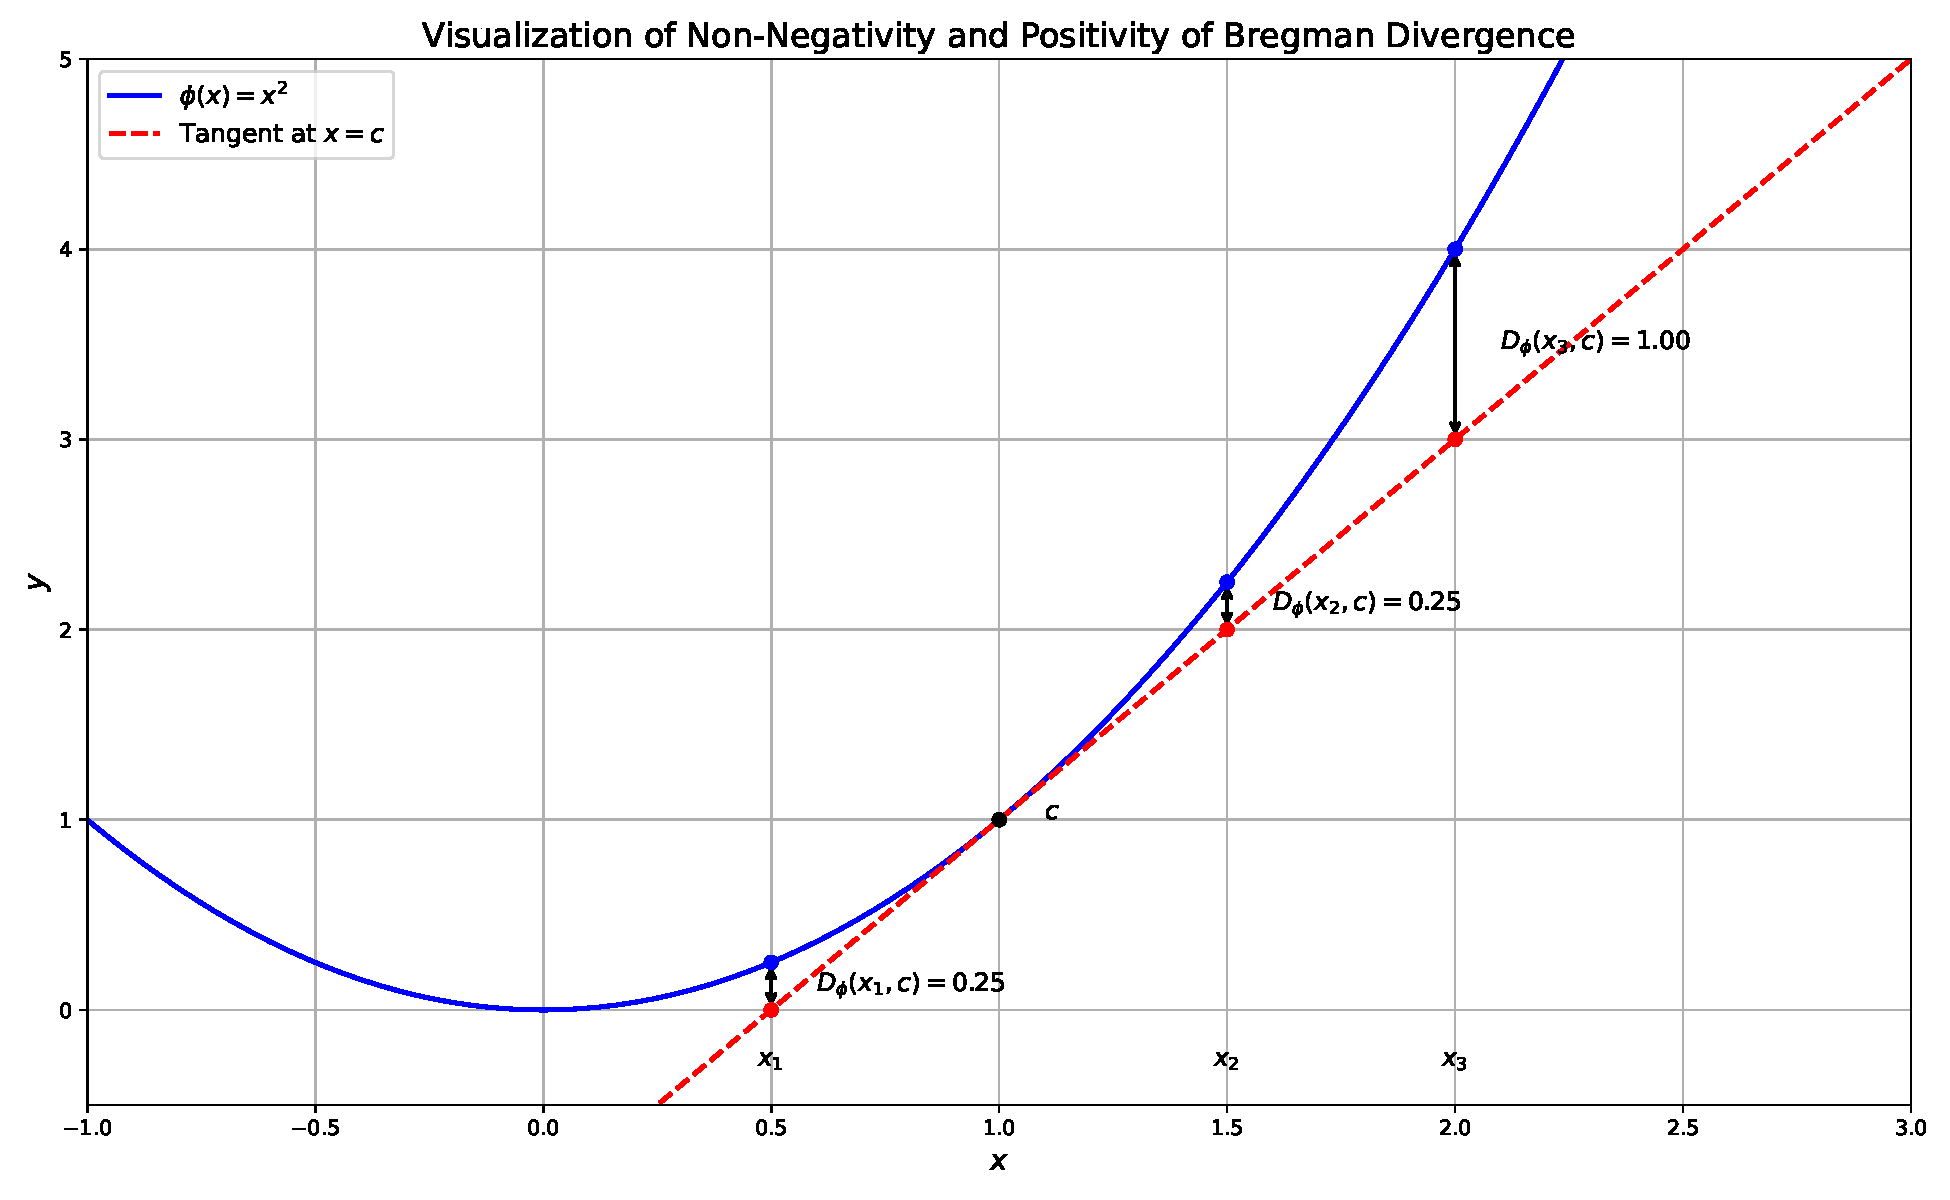
\includegraphics[width=\textwidth]{non-neg.pdf} % Adjust width as needed
    \caption{Неотрицательность и позитивность дивергенции Брэгмана}
    \label{fig:non-neg}
\end{figure}

\paragraph{Инвариантность к добавлению аффинной функции}\label{par:affine_difference}
\begin{equation}
    D_\psi (p,q) = D_\phi(p,q) \Longleftrightarrow \psi(x) = \phi (x) \langle a, x \rangle + b, \text{where}\ a \in \mathbb{R}^n \wedge \ b \in \mathbb{R}
\end{equation}
Дивергенция Брэгмана остаётся неизменной, если порождающая функция $\phi$ модифицируется путём добавления аффинного члена. Это свойство подчёркивает внутреннюю природу дивергенции, не зависящую от линейных сдвигов или постоянных смещений~\cite{Harremoes2017}. Иными словами, дивергенция Брэгмана инвариантна при добавлении аффинной функции к выпуклой функции. Рассмотрим рисунок~\ref{fig:affinity} на странице~\pageref{fig:affinity}.


\begin{figure}[h]
    \centering
    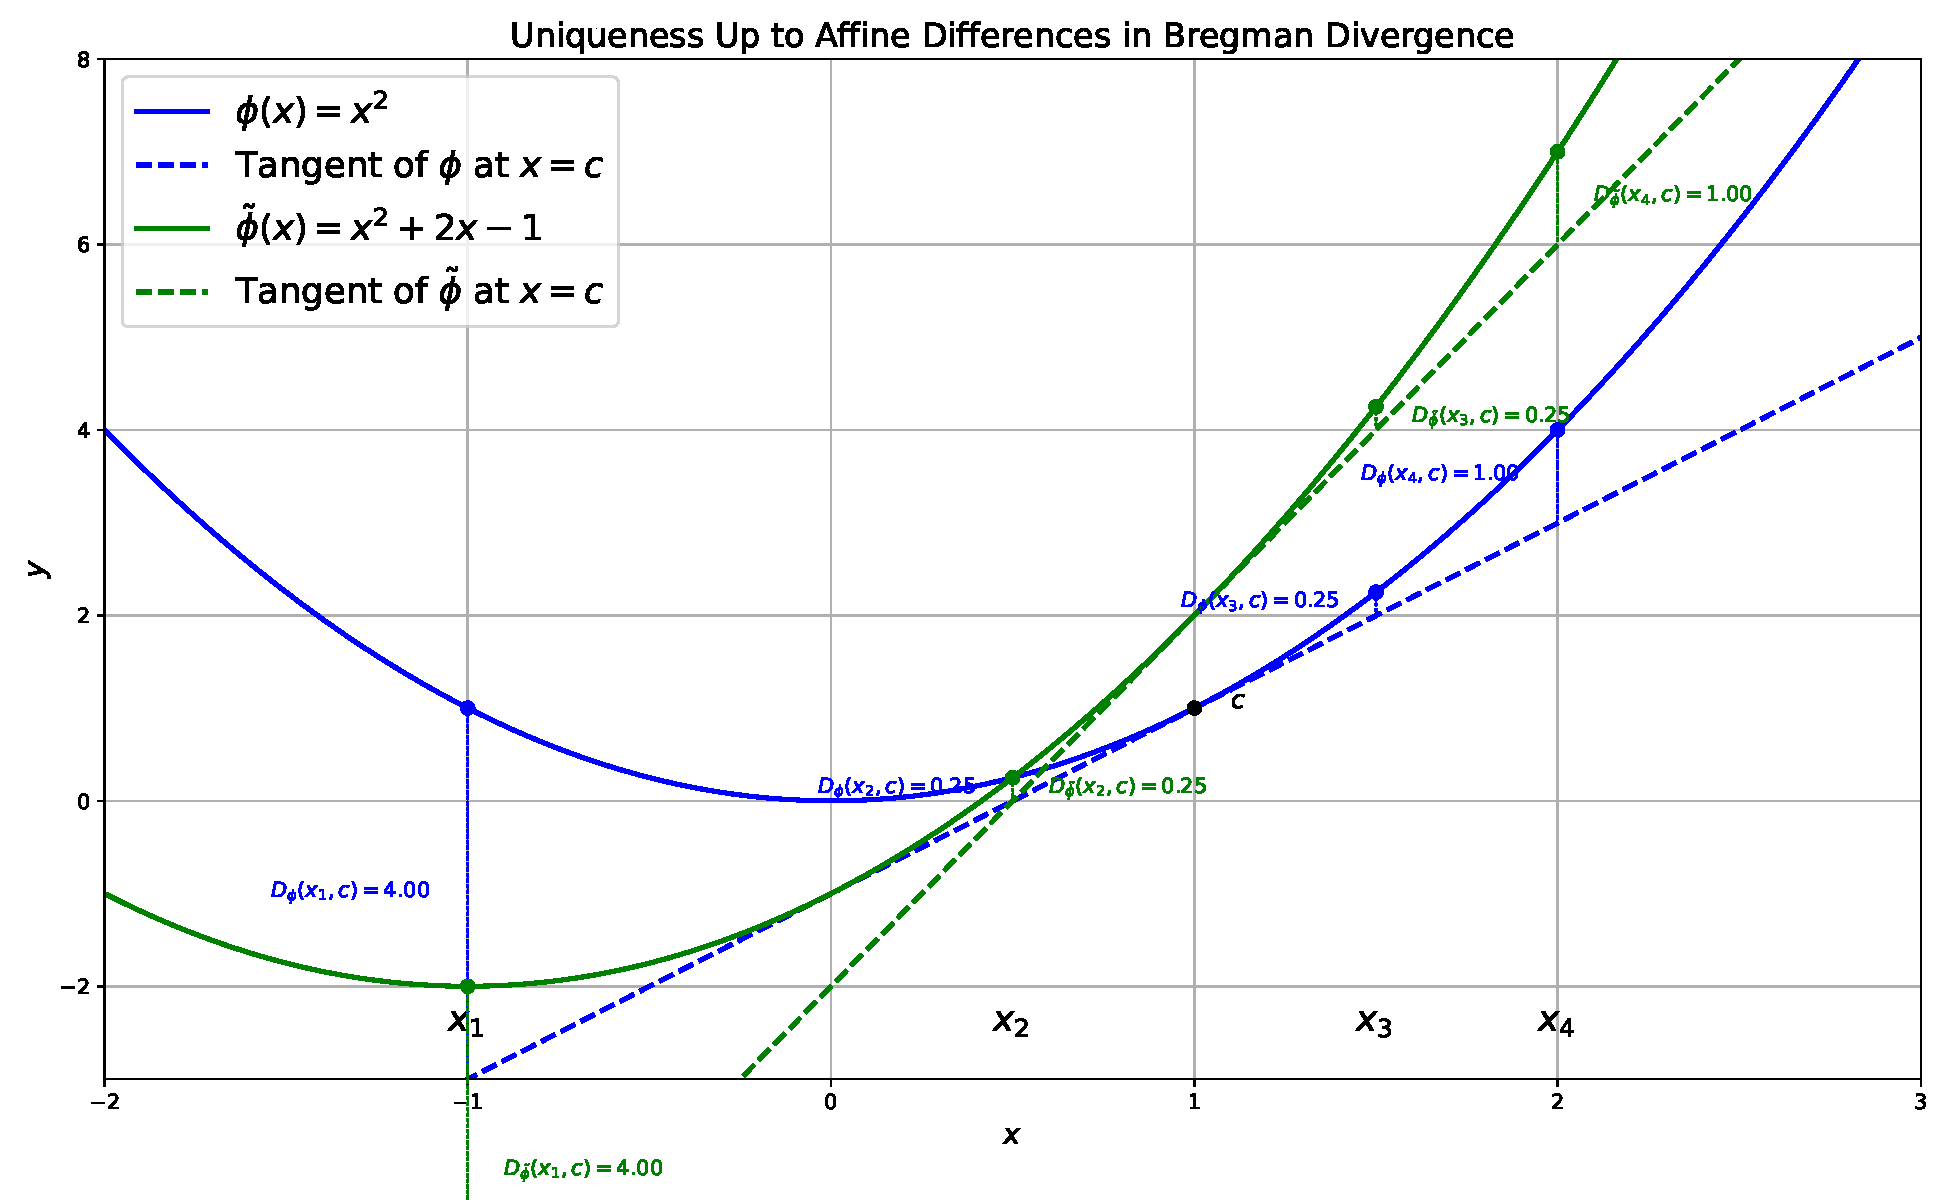
\includegraphics[width=\textwidth]{affinnity.pdf} % Adjust width as needed
    \caption{Инвариантность к добавлению аффинной функции}
    \label{fig:affinity}
\end{figure}

\paragraph{Выпуклость} $D_\phi(p,q)$ является выпуклой по первому аргументу p, но не обязательно по второму аргументу q~\cite{Nielsen2017}. Это свойство выпуклости очень важно для алгоритмов оптимизации, поскольку оно обеспечивает существование единственного минимума при минимизации расхождения относительно первого аргумента~\cite{Frigyik2008a}.
\paragraph{Линейность}\label{par:linearity}
Для любых двух строго выпуклых функций дифференцируемых функций $\phi_{1}$ и $\phi_{1}$ и любых $a,\beta > 0$,
\begin{equation}
    D_{\alpha \phi_{1} + \beta \phi_{2}}(p,q) = \alpha D_{\phi_{1}} (p,q) + \beta D_{\phi_{2}} (p,q)
\end{equation}
Линейность дивергенций Брэгмана позволяет комбинировать несколько дивергенций, порождённых различными функциями~\cite{Reid2013}.
\paragraph{Двойственность}\label{par:duality}
Для любой строго выпуклой и дифференцируемой функции $\phi$ и её выпуклой сопряжённой $\phi^{*}$
\begin{equation}
    D_{\phi}(p,q) = D_{\phi^{*}}(\triangledown \phi(q), \triangledown \phi(p))
\end{equation}
Дивергенция Брегмана имеет двойственную связь со своей выпуклой сопряжённой, соединяя дивергенцию в начальном пространстве с соответствующей дивергенцией в двойственном пространстве~\cite{Nielsen2019}.
\paragraph{Среднее как минимизатор}\label{par:mean_as_minimizer}
Для любой $q \in S$ и любого случайного вектора $X$, принимающего значения в $S$:
\begin{equation}
    q =  E[X] \Longrightarrow E[D_\phi (X,q)] = min
\end{equation}
Ожидаемое расхождение Брэгмана между случайным вектором и фиксированной точкой минимизируется, если фиксированная точка является средним значением случайного вектора. Это свойство подчёркивает связь между дивергенциями Брегмана и такими статистическими понятиями, как матожидание и среднее~\cite{Iyer2012}. Этот вывод обобщает хрестоматийный результат о том, что среднее значение множества минимизирует суммарную квадратичную ошибку для элементов этого множества~\cite{Nielsen2007a}.  Этот результат был доказан для случая векторов~\cite{JMLR:v6:banerjee05b}, и расширен на случай функций (распределений) в работе~\cite{Frigyik2008}. Этот результат важен, поскольку он дополнительно обосновывает использование среднего значения в качестве представителя случайного множества, особенно в Байесовских оценках~\cite{Jiao2014}.
\paragraph{Сферы Брэгмана ограничены и компактны, если X замкнут}\label{par:bregman_balls}
Сфера (шар) Брэгмана радиусом $r$ с центром в $c$ определяется как:
\begin{equation}
    {x \in S:D_{\phi}(x,c) \leq r}
\end{equation}
и является ограниченной и компактной, если множество $S$ закрытое~\cite{Nielsen2007}. Это свойство гарантирует, что множество точек, находящихся в пределах определённого расхождения Брегмана от заданного центра~\cite{Nielsen2011}, является хорошо управляемым~\cite{Nielsen2006}, что облегчает анализ и оптимизацию в пределах этого множества~\cite{Boissonnat2010}.
\paragraph{Теорема косинусов}\label{par:cosine_rule}
\begin{equation}
    \forall p,q,z \in S,\ D_{\phi}(p,z) = D_{\phi}(q,z) - \langle \triangledown \phi (z) - \triangledown \phi (q), p -q \rangle
\end{equation}
Дивергенция Брэгмана удовлетворяет обобщённому правилу косинусов, связывая дивергенции между тремя точками способом, напоминающим классический закон косинусов в евклидовой геометрии~\cite{Adamcik2014}.

\section{Практическое применение}\label{sec:Case}






\printbibliography

\end{document}
